\documentclass[12pt]{article}
 
\usepackage[margin=1in]{geometry}
\usepackage{amsmath,amsthm,amssymb}
\usepackage{fancyhdr}
\usepackage{hyperref}
\pagestyle{fancy}
\usepackage{graphicx}
\newcommand{\N}{\mathbb{N}}
\newcommand{\R}{\mathbb{R}}
\newcommand{\Z}{\mathbb{Z}}
\newcommand{\Q}{\mathbb{Q}}
 
\newenvironment{theorem}[2][Theorem]{\begin{trivlist}
\item[\hskip \labelsep {\bfseries #1}\hskip \labelsep {\bfseries #2.}]}{\end{trivlist}}
\newenvironment{lemma}[2][Lemma]{\begin{trivlist}
\item[\hskip \labelsep {\bfseries #1}\hskip \labelsep {\bfseries #2.}]}{\end{trivlist}}
\newenvironment{exercise}[2][Exercise]{\begin{trivlist}
\item[\hskip \labelsep {\bfseries #1}\hskip \labelsep {\bfseries #2.}]}{\end{trivlist}}
\newenvironment{problem}[2][Problem]{\begin{trivlist}
\item[\hskip \labelsep {\bfseries #1}\hskip \labelsep {\bfseries #2.}]}{\end{trivlist}}
\newenvironment{question}[2][Question]{\begin{trivlist}
\item[\hskip \labelsep {\bfseries #1}\hskip \labelsep {\bfseries #2.}]}{\end{trivlist}}
\newenvironment{corollary}[2][Corollary]{\begin{trivlist}
\item[\hskip \labelsep {\bfseries #1}\hskip \labelsep {\bfseries #2.}]}{\end{trivlist}}
 
\begin{document}
 
\title{Lab 5: Congestion Control for Audio Streaming}
\author{Duc Viet Le\\
 CS536}
 
\maketitle
 
\begin{problem}{1} \ \\
As we discussed in class, method D has the best result. Below are plots for each method:
\\
\textbf{Method A} \\
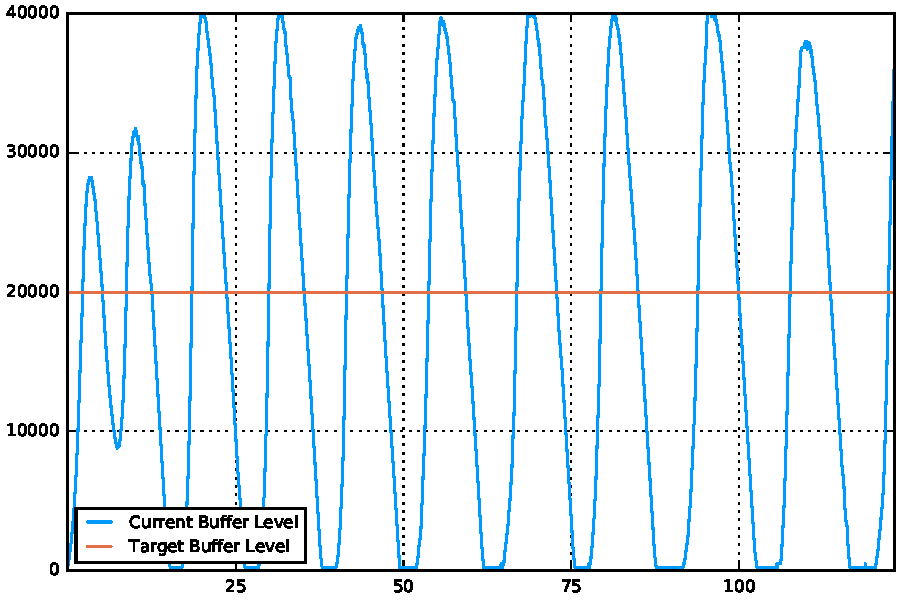
\includegraphics[scale = .5]{listen0.pdf}
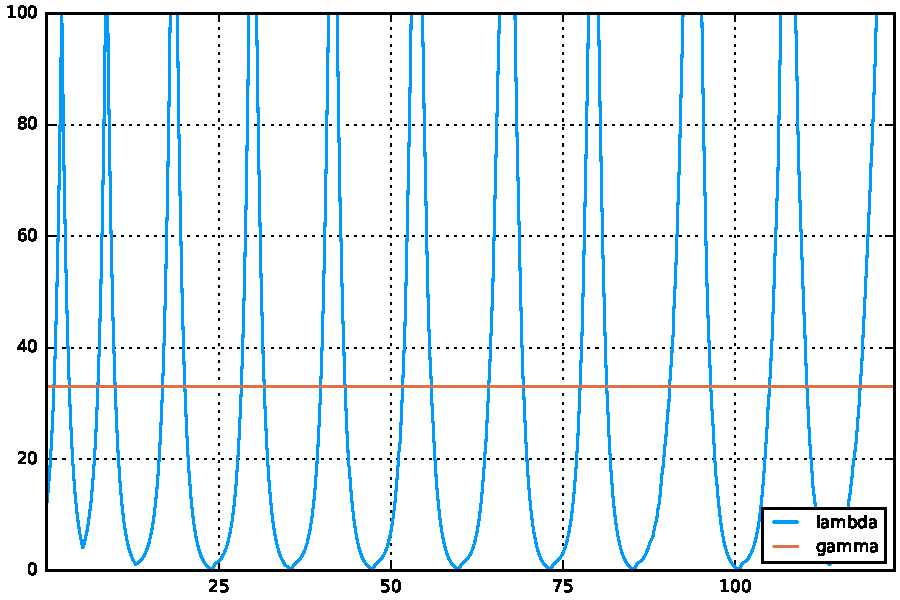
\includegraphics[scale = .5]{stream0.pdf}
\\
\textbf{Method B} \\
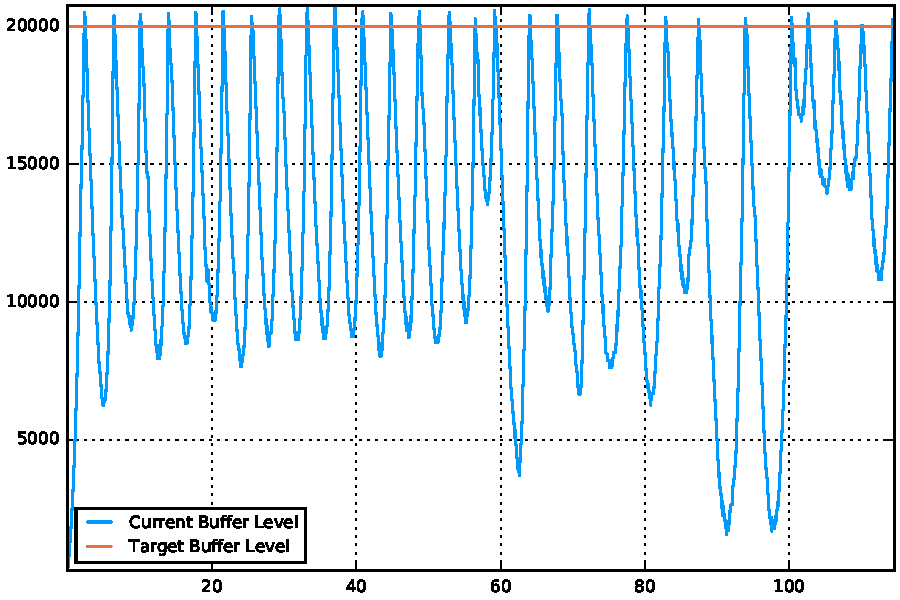
\includegraphics[scale = .5]{listen1.pdf}
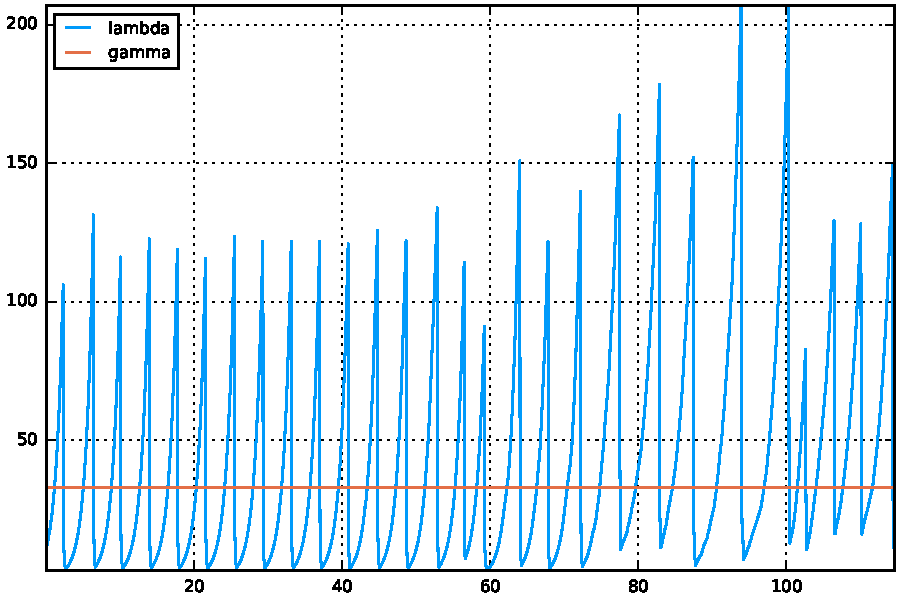
\includegraphics[scale = .5]{stream1.pdf}
\\
\textbf{Method C} \\
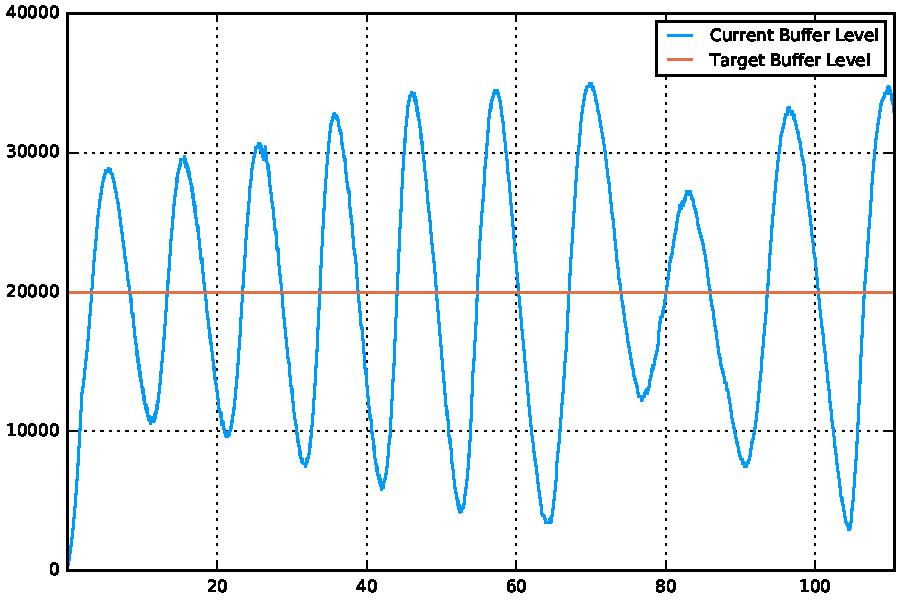
\includegraphics[scale = .5]{listen2.pdf}
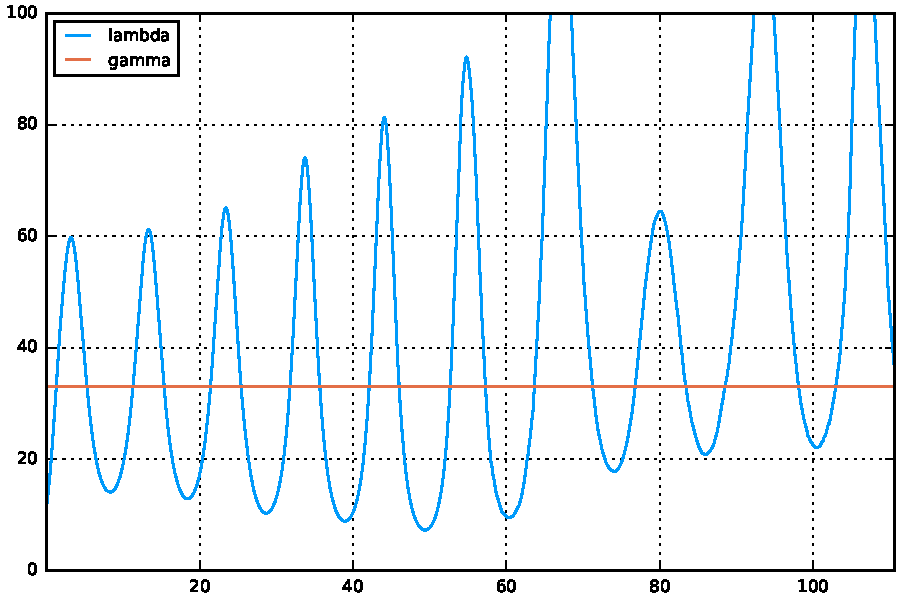
\includegraphics[scale = .5]{stream2.pdf}
\\
\textbf{Method D} \\
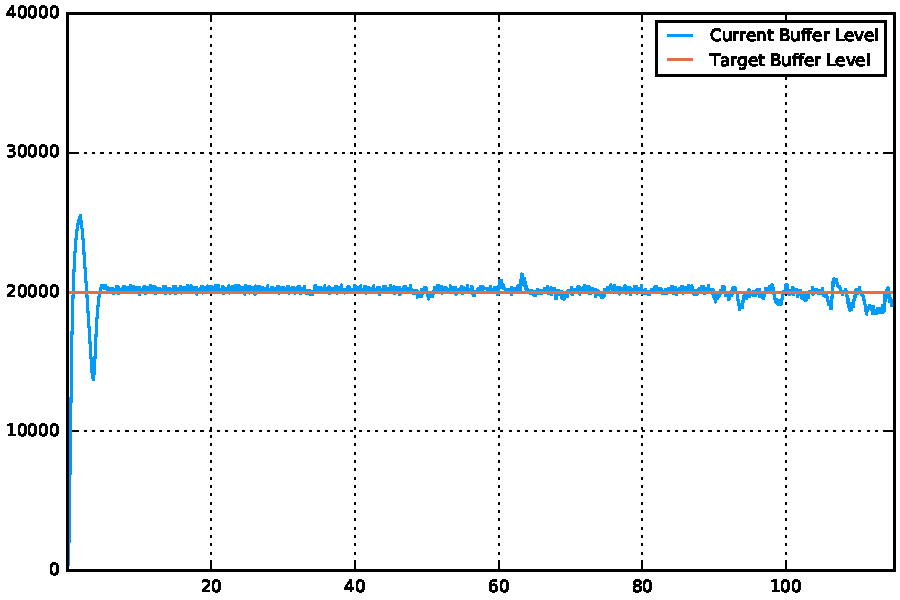
\includegraphics[scale = .5]{listen3.pdf}
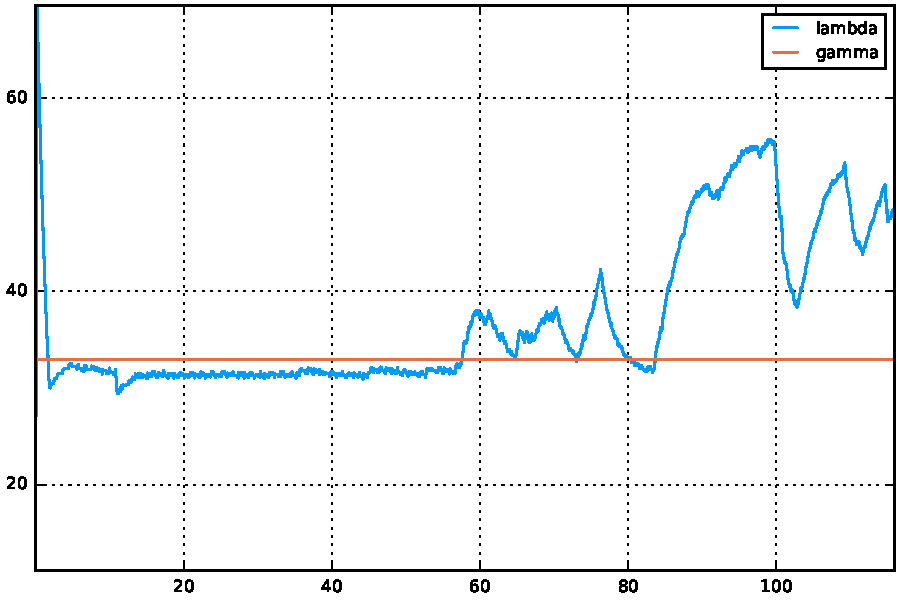
\includegraphics[scale = .5]{stream3.pdf}
\\
\textit{Discussion:}

\end{problem}

\end{document}
